\documentclass[8pt,a4paper]{article}
\usepackage[margin=0.4cm]{geometry}
\usepackage{multicol}
\usepackage{amsmath,amssymb}
\usepackage{enumitem}
\usepackage{array}
\usepackage{graphicx}
\usepackage{CJKutf8}

\setlength{\columnseprule}{0.3pt}
\setlength{\columnsep}{0.3cm}
\setlist{nosep,leftmargin=*}
\pagestyle{empty}
\setlength{\parindent}{0pt}
\setlength{\parskip}{0.5pt}
\setlength{\abovedisplayskip}{0pt}
\setlength{\belowdisplayskip}{0pt}
\setlength{\abovedisplayshortskip}{0pt}
\setlength{\belowdisplayshortskip}{0pt}

\newcommand{\mysection}[1]{\vspace{2pt}\textbf{#1}\vspace{1pt}}
\newcommand{\mysubsection}[1]{\vspace{1pt}\textbf{#1:}\vspace{0.5pt}}

\begin{document}
\begin{CJK}{UTF8}{min}

\begin{multicols}{3}

\mysection{PROBLEM 1: CONVEX SET \& CONVEX FUNCTION}

\textbf{凸集合の定義}: 集合$S \subseteq \mathbb{R}^n$が凸集合であるとは、任意の$\boldsymbol{x}, \boldsymbol{y} \in S$と任意の$\alpha \in [0,1]$に対して
\[
(1-\alpha)\boldsymbol{x} + \alpha\boldsymbol{y} \in S
\]
が成り立つこと。\\
\textbf{意味}: 集合内の任意の2点を結ぶ線分上の点も全て集合に含まれる

\textbf{凸関数の定義}: 凸集合$S$上で定義された関数$f: S \to \mathbb{R}$が凸関数であるとは、任意の$\boldsymbol{x}, \boldsymbol{y} \in S$と任意の$\alpha \in [0,1]$に対して
\[
f((1-\alpha)\boldsymbol{x} + \alpha\boldsymbol{y}) \leq (1-\alpha)f(\boldsymbol{x}) + \alpha f(\boldsymbol{y})
\]
が成り立つこと。\\
\textbf{意味}: 関数のグラフ上の任意の2点を結ぶ線分が、関数のグラフの上側にある

\mysection{PROBLEM 3: EXTREME POINTS \& RAYS}
\begin{itemize}
    \item A: bounded な多面体には extreme ray（方向）= 無限に伸びる方向 が存在しない。だからこれは 間違い。
    \item B: 
    \begin{itemize}
        \item bounded polyhedron $\to$ extreme points 必ず存在する（=polytope）
        \item extreme point が無い $\to$ bounded ではない $\to$ 必ず unbounded
    \end{itemize}
    \item C: 空でない polyhedron 内の任意の点は、
    \begin{itemize}
        \item bounded の場合 $\to$ extreme point の凸結合だけで表せる。
        \item unbounded の場合 $\to$ extreme point の凸結合 + extreme ray の非負結合で表せる。
    \end{itemize}
\end{itemize}

\mysection{PROBLEM 4: RELAXATION PROBLEM}

\textbf{緩和問題の定義（最小化問題）}: 元の問題の実行可能領域を拡大した問題

\textbf{性質}:
\begin{itemize}
    \item 元の問題の実行可能領域 $\subseteq$ 緩和問題の実行可能領域
    \item 緩和問題の最適値 $\leq$ 元の問題の最適値（下界を与える）
\end{itemize}

\textbf{緩和の作り方}:
\begin{itemize}
    \item 制約を削除または緩める（例: $g(x) \geq 0$ $\to$ $g(x) \geq -1$）
    \item 整数制約を外す（例: $x \in \mathbb{Z}$ $\to$ $x \in \mathbb{R}$）
    \item 目的関数を変更（例: $f(x)$ $\to$ $f(x) + h(x)$、ただし$h(x) \geq 0$）
\end{itemize}

\mysection{PROBLEM 5: DUALITY}
\begin{align*}
\text{minimize} \quad & 3x_1 + 5x_2 + 7x_3 \\
\text{subject to} \quad & -x_1 + 3x_2 = 5 \\
& 2x_1 - x_2 + 3x_3 \geq 6 \\
& x_3 \leq 7 \\
& x_1 \geq 0, \quad x_2 \leq 0, \quad x_3 \text{ free}
\end{align*}

まず、各制約に対してラグランジュ乗数 $y_1$, $y_2$, $y_3$ を導入する。
制約の符号に基づき、それぞれの双対変数は次のようになる：
\begin{itemize}
    \item 等式制約（$-x_1 + 3x_2 = 5$）に対応する $y_1$ は符号制限なし（free）
    \item 「$\geq$」制約（$2x_1 - x_2 + 3x_3 \geq 6$）に対応する $y_2$ は $y_2 \geq 0$
    \item 「$\leq$」制約（$x_3 \leq 7$）に対応する $y_3$ は $y_3 \leq 0$
\end{itemize}
これらを用いてラグランジュ関数 $L(x, y)$ を構成すると、
\begin{align*}
L(x, y) &= 3x_1 + 5x_2 + 7x_3 \\
&\quad - y_1(-x_1 + 3x_2 - 5) \\
&\quad - y_2(2x_1 - x_2 + 3x_3 - 6) \\
&\quad - y_3(x_3 - 7)
\end{align*}
展開し、$x_1$, $x_2$, $x_3$ に関する係数をまとめると、
\begin{align*}
L(x,y) &= (3 + y_1 - 2y_2)x_1 \\
&\quad + (5 - 3y_1 + y_2)x_2 \\
&\quad + (7 - 3y_2 - y_3)x_3 \\
&\quad + 5y_1 + 6y_2 + 7y_3
\end{align*}
次に、ラグランジュ双対関数 $g(y)$ を求めるために、
\[
g(y) = \inf_x L(x,y)
\]
を考える。

この下界が有限になるためには、変数 $x$ の符号制約により以下の条件が必要となる：
\begin{itemize}
    \item $x_1 \geq 0$ なので、係数 $(3 + y_1 - 2y_2) \geq 0$
    \item $x_2 \leq 0$ なので、係数 $(5 - 3y_1 + y_2) \leq 0$
    \item $x_3$ は自由変数なので、係数 $(7 - 3y_2 - y_3) = 0$
\end{itemize}
これらの条件が満たされるとき、$L(x,y)$ の $\inf$ は、係数部分が 0 になる点（つまり $x=0$）で達成される。
したがって、双対関数は次のように定まる：
\[
g(y) = 5y_1 + 6y_2 + 7y_3
\]
以上より、双対問題（Dual）は次のようになる：
$\begin{aligned}
\text{maximize} \quad & 5y_1 + 6y_2 + 7y_3 \\
\text{subject to} \quad & -y_1 + 2y_2 \leq 3 \\
& 3y_1 - y_2 \geq 5 \\
& 3y_2 + y_3 = 7 \\
& y_1 \text{ free}, \quad y_2 \geq 0, \quad y_3 \leq 0
\end{aligned}$

\mysection{PROBLEM 6: DUALITY THEOREMS}

\textbf{弱双対定理}: 主問題と双対問題のいずれか一方が\textbf{非有界}ならば他方は\textbf{実行不可能}である。
\begin{itemize}
    \item 逆は成り立たない（実行不能 $\nRightarrow$ 非有解）
    \item \textbf{注意}: 片方が実行不能の場合、もう片方は「非有解」か「実行不能」のどちらかである（両方実行不能もあり得る）。
\end{itemize}

\textbf{強双対定理}: 主問題に最適解$x^*$が存在すれば双対問題にも最適解$y^*$が存在し目的関数の値は一致する。

\mysection{PROBLEM 7: ROBUST OPTIMIZATION}

\textbf{問題設定}:
\[
\min \boldsymbol{c}^T \boldsymbol{x} \quad \text{s.t.} \quad \boldsymbol{a}^T \boldsymbol{x} \leq b, \quad \forall \boldsymbol{a} \in U
\]
パラメータ $\boldsymbol{a}$ は不確実性集合 $U = \{\boldsymbol{a} \in \mathbb{R}^n \mid B\boldsymbol{a} \leq \boldsymbol{d}\}$ に含まれる。\\
\textbf{注意}: $b$はスカラー（1つの制約式の場合）

\textbf{最悪ケースへの変換}:
制約 $\boldsymbol{a}^T \boldsymbol{x} \leq b$ が全ての $\boldsymbol{a} \in U$ で成り立つには、$\boldsymbol{a}^T \boldsymbol{x}$ の最大値（最悪ケース）でも成り立てば良い。
\[
\max_{\boldsymbol{a} \in U} (\boldsymbol{a}^T \boldsymbol{x}) \leq b
\]

\textbf{双対問題への書き換え}:
内側の最大化問題を考える（\textbf{注意}: $\boldsymbol{x}$ は定数、$\boldsymbol{a}$ が変数）。
\[
\text{(P)}: \quad \max_{\boldsymbol{a}} \boldsymbol{x}^T \boldsymbol{a} \quad \text{s.t.} \quad B\boldsymbol{a} \leq \boldsymbol{d}
\]
これを双対問題 (D) に変換する。
\[
\text{(D)}: \quad \min_{\boldsymbol{y}} \boldsymbol{d}^T \boldsymbol{y} \quad \text{s.t.} \quad B^T \boldsymbol{y} = \boldsymbol{x}, \quad \boldsymbol{y} \geq \mathbf{0}
\]
\begin{itemize}
    \item \textbf{目的関数}: $\max \boldsymbol{x}^T \boldsymbol{a} \to \min \boldsymbol{d}^T \boldsymbol{y}$
    \item \textbf{制約}: 変数 $\boldsymbol{a}$ に符号制約なし $\to$ 双対制約は等式 $B^T \boldsymbol{y} = \boldsymbol{x}$
    \item \textbf{符号}: $B\boldsymbol{a} \leq \boldsymbol{d}$ $\to$ 双対変数 $\boldsymbol{y} \geq \mathbf{0}$
\end{itemize}

\textbf{強双対性}: 最適値が一致するので、元の制約は $\boldsymbol{d}^T \boldsymbol{y} \leq b$ と書き換えられる。

\textbf{最終的な定式化 (LP)}:\\
$\min \boldsymbol{c}^T \boldsymbol{x}$ s.t. $\boldsymbol{d}^T \boldsymbol{y} \leq b$, $B^T \boldsymbol{y} = \boldsymbol{x}$, $\boldsymbol{y} \geq \mathbf{0}$

\mysection{PROBLEM 7 (EXAMPLE): ROBUST CONSTRAINT}

\textbf{問題}: $\boldsymbol{a}^T \boldsymbol{x} \geq b$, $\forall \boldsymbol{a} \in U = \{\boldsymbol{a} \in [0,1]^n \mid C\boldsymbol{a} \leq \boldsymbol{d}\}$ を書き換え

\textbf{ステップ1}: 最悪ケース $\min_{\boldsymbol{a} \in U} \boldsymbol{a}^T \boldsymbol{x} \geq b$\\
内側問題: $\min \boldsymbol{x}^T \boldsymbol{a}$ s.t. $C\boldsymbol{a} \leq \boldsymbol{d}$, $\boldsymbol{a} \leq \boldsymbol{e}$, $\boldsymbol{a} \geq \mathbf{0}$（$\boldsymbol{x}$は定数、$\boldsymbol{a}$が変数）

\textbf{ステップ2}: ラグランジュ緩和\\
ラグランジュ関数 $L(\boldsymbol{a}, \boldsymbol{y}, \boldsymbol{z}) = \boldsymbol{x}^T \boldsymbol{a} + \boldsymbol{y}^T (C\boldsymbol{a} - \boldsymbol{d}) + \boldsymbol{z}^T (\boldsymbol{a} - \boldsymbol{e})$\\
$= (\boldsymbol{x} + C^T \boldsymbol{y} + \boldsymbol{z})^T \boldsymbol{a} - \boldsymbol{d}^T \boldsymbol{y} - \boldsymbol{e}^T \boldsymbol{z}$\\
ここで $\boldsymbol{y}, \boldsymbol{z} \geq \mathbf{0}$。\\
$\min_{\boldsymbol{a} \geq \mathbf{0}} L$ が有限（$-\infty$にならない）であるためには、$\boldsymbol{a}$ の係数が非負である必要がある。\\
$\implies \boldsymbol{x} + C^T \boldsymbol{y} + \boldsymbol{z} \geq \mathbf{0}$\\
このとき $\min L = -\boldsymbol{d}^T \boldsymbol{y} - \boldsymbol{e}^T \boldsymbol{z}$。\\
よって双対問題は $\max (-\boldsymbol{d}^T \boldsymbol{y} - \boldsymbol{e}^T \boldsymbol{z})$。

\textbf{ステップ3}: 強双対より最大値 $\geq b$\\
$-\boldsymbol{d}^T \boldsymbol{y} - \boldsymbol{e}^T \boldsymbol{z} \geq b \iff \boldsymbol{d}^T \boldsymbol{y} + \boldsymbol{e}^T \boldsymbol{z} + b \leq 0$

\textbf{正解 (C)}: $\boldsymbol{d}^T \boldsymbol{y} + \boldsymbol{e}^T \boldsymbol{z} + b \leq 0$, $\boldsymbol{x} + C^T \boldsymbol{y} + \boldsymbol{z} \geq \mathbf{0}$, $\boldsymbol{y}, \boldsymbol{z} \geq \mathbf{0}$

\mysection{PROBLEM 9: CUTTING STOCK \& COLUMN GENERATION}

\textbf{列生成法}: 変数が膨大な場合、全て列挙せず改善する変数のみ逐次生成（Gilmore \& Gomory, 1961）

\textbf{MP（マスター問題）}: 全てのパターンを含む元の問題
\begin{align*}
\text{最小化:} \quad & \sum_{j=1}^n x_j \\
\text{条件:} \quad & \sum_{j=1}^n a_{ij} x_j \geq d_i, \quad i = 1, \ldots, m \\
& \sum_{i=1}^m a_{ij} l_i \leq L \quad \text{(パターン条件)} \\
& x_j \in \mathbb{Z}_+
\end{align*}
※ $n$ は全パターン数（膨大）

\textbf{MPの重要な性質}:
\begin{itemize}
    \item \textbf{実行可能性}: RMPの実行可能解（選択された変数以外を0としたもの）は、MPにとっても実行可能
    \item \textbf{双対性の利用}: RMPの双対変数は、次にどの変数を追加すべきかを判断するために不可欠
\end{itemize}

\textbf{RMP（制限マスター問題）}: 現在生成済みのパターン集合 $I$ のみを含む問題
\begin{align*}
\text{最小化:} \quad & \sum_{j \in I} x_j \\
\text{条件:} \quad & \sum_{j \in I} a_{ij} x_j \geq d_i, \quad i = 1, \ldots, m \\
& x_j \geq 0 \quad \text{(LP緩和)}
\end{align*}
\textbf{出力}: 暫定解 $x$ と双対変数 $\mathbf{y}^* = (y_1^*, \ldots, y_m^*)$

\textbf{Pricing Problem（価格付け問題）}: 被約費用が負になる新しい列を探す
\begin{align*}
\text{最大化:} \quad & \sum_{i=1}^m y_i^* a_i' \\
\text{条件:} \quad & \sum_{i=1}^m l_i a_i' \leq L, \quad a_i' \in \mathbb{Z}_+
\end{align*}
\textbf{判定}: 最適値 $> 1$ なら新パターン $\mathbf{p}^*$ をRMPに追加、$\leq 1$ なら終了

\textbf{列生成の流れ}:
\begin{enumerate}
    \item 初期: $I = \{\mathbf{p}_i = (0,\ldots,\lfloor L/l_i \rfloor,\ldots,0) : i=1,\ldots,m\}$
    \item \textbf{RMP}を解く $\to$ 双対解 $\mathbf{y}^*$ を取得
    \item \textbf{Pricing Problem}を解く（動的計画法）
    \item 最適値 $\leq 1$ なら終了、そうでなければ新パターンを$I$に追加して2へ
\end{enumerate}

\textbf{動的計画法}: $\bar{l} = \min l_i$ として
\begin{align*}
f(v) &= \max_{1 \leq i \leq m, \, l_i \leq v} \{ f(v-l_i) + y_i^* \}, \quad v = \bar{l},\ldots,L \\
f(v) &= 0, \quad 0 \leq v < \bar{l}
\end{align*}

\textbf{3つの違い}:
\begin{itemize}
    \item \textbf{MP}: 全パターンを含む理想的な問題（解けない）
    \item \textbf{RMP}: 既知パターンで最適配分を決める「調整役」（LP）
    \item \textbf{Pricing}: 改善する新パターンを探す「生成役」（ナップサック）
\end{itemize}

\mysection{PROBLEM 10: DANTZIG-WOLFE DECOMPOSITION}

\textbf{Dantzig-Wolfe分解}: 特殊構造を持つ大規模LPを列生成で解く手法

\textbf{元の問題（LP）}:
\begin{align*}
\text{最小化:} \quad & \boldsymbol{c}^T \boldsymbol{x} \\
\text{条件:} \quad & \boldsymbol{D}\boldsymbol{x} = \boldsymbol{b}_0 \quad \text{(難しい制約)} \\
& \boldsymbol{F}\boldsymbol{x} = \boldsymbol{b} \quad \text{(簡単な制約)} \\
& \boldsymbol{x} \geq \mathbf{0}
\end{align*}

\textbf{ステップ1: 制約の分離}
多面体 $P = \{\boldsymbol{x} \mid \boldsymbol{F}\boldsymbol{x} = \boldsymbol{b}, \boldsymbol{x} \geq \mathbf{0}\}$ を定義
\begin{align*}
\text{最小化:} \quad & \boldsymbol{c}^T \boldsymbol{x} \\
\text{条件:} \quad & \boldsymbol{D}\boldsymbol{x} = \boldsymbol{b}_0 \\
& \boldsymbol{x} \in P
\end{align*}

\textbf{ステップ2: 極点表現への変換}
$P$の極点を $\boldsymbol{x}^1, \ldots, \boldsymbol{x}^N$ とすると、任意の $\boldsymbol{x} \in P$ は
\begin{align*}
\boldsymbol{x} &= \sum_{i=1}^N \lambda_i \boldsymbol{x}^i \\
\sum_{i=1}^N \lambda_i &= 1, \quad \lambda_i \geq 0
\end{align*}

\textbf{MP（マスター問題）}:
\begin{align*}
\text{最小化:} \quad & \sum_{i=1}^N \lambda_i (\boldsymbol{c}^T \boldsymbol{x}^i) \\
\text{条件:} \quad & \sum_{i=1}^N \lambda_i (\boldsymbol{D}\boldsymbol{x}^i) = \boldsymbol{b}_0 \\
& \sum_{i=1}^N \lambda_i = 1 \\
& \lambda_i \geq 0
\end{align*}
※ $N$ は極点数（膨大、$2^n$など）

\textbf{RMP（制限マスター問題）}: 現在生成済みの極点集合 $I$ のみを含む
\begin{align*}
\text{最小化:} \quad & \sum_{i \in I} \lambda_i (\boldsymbol{c}^T \boldsymbol{x}^i) \\
\text{条件:} \quad & \sum_{i \in I} \lambda_i (\boldsymbol{D}\boldsymbol{x}^i) = \boldsymbol{b}_0 \\
& \sum_{i \in I} \lambda_i = 1 \\
& \lambda_i \geq 0
\end{align*}
\textbf{出力}: 暫定解 $\hat{\lambda}$ と双対変数 $[\hat{\boldsymbol{y}}^T, \hat{r}]$

\textbf{Subproblem（サブ問題）}: 被約費用の最小値を求める
\begin{align*}
Z = \min_{i=1,\ldots,N} \quad & \left\{ \boldsymbol{c}^T \boldsymbol{x}^i - \hat{\boldsymbol{y}}^T \boldsymbol{D}\boldsymbol{x}^i - \hat{r} \right\}
\end{align*}
サブ問題として定式化すると：
\begin{align*}
Z = \min_{\boldsymbol{x} \in P} \quad & \left\{ (\boldsymbol{c}^T - \hat{\boldsymbol{y}}^T \boldsymbol{D}) \boldsymbol{x} - \hat{r} \right\}
\end{align*}
\textbf{判定}: $Z \geq 0$ なら最適（終了）、$Z < 0$ なら被約費用最小の列をRMPに追加

\textbf{列生成の流れ}:
\begin{enumerate}
    \item 初期: 極点を数個選んで$I$を初期化
    \item \textbf{RMP}を解く $\to$ 双対解 $[\hat{\boldsymbol{y}}, \hat{r}]$ を取得
    \item \textbf{Subproblem}を解いて被約費用の最小値$Z$を計算
    \item $Z \geq 0$ なら終了、$Z < 0$ なら被約費用最小の極点を$I$に追加して2へ
\end{enumerate}

\textbf{重要な性質}:
\begin{itemize}
    \item \textbf{極点表現}: 有界多面体（polytope）の任意の点は極点の凸結合で表現可能
    \item \textbf{等価性}: MPの最適解から元の問題（LP）の最適解を復元可能
    \item \textbf{双対変数}: $\hat{\boldsymbol{y}}$は難しい制約の影の価格、$\hat{r}$は凸結合制約の影の価格
\end{itemize}

\mysection{PROBLEM 13: L1 \& L2 NORMS}

\textbf{L1ノルム（1-norm）}:
\begin{itemize}
    \item \textbf{別名}: Manhattan norm, Taxicab norm
    \item \textbf{定義}: $\|\boldsymbol{x}\|_1 = \sum_{i=1}^n |x_i|$
\end{itemize}

\textbf{L2ノルム（2-norm）}:
\begin{itemize}
    \item \textbf{別名}: Euclidean norm
    \item \textbf{定義}: $\|\boldsymbol{x}\|_2 = \sqrt{\sum_{i=1}^n x_i^2} = \sqrt{\boldsymbol{x}^T \boldsymbol{x}}$
\end{itemize}

\textbf{一般化}: $p$-ノルム $\|\boldsymbol{x}\|_p = \left(\sum_{i=1}^n |x_i|^p\right)^{1/p}$

\textbf{最小二乗問題 (Least Square Problem) の例}:
$\min_{x} \|A\boldsymbol{x} - \boldsymbol{b}\|_2^2$。$A = \begin{bmatrix} 2 & 3 \\ 0 & 1 \\ 0 & 0 \end{bmatrix}, \boldsymbol{b} = \begin{bmatrix} 2 \\ 3 \\ 1 \end{bmatrix}$

\textbf{解法}: 正規方程式 $A^T A \boldsymbol{x} = A^T \boldsymbol{b}$ を解く。
\begin{enumerate}
    \item $A^T A = \begin{bmatrix} 2 & 0 & 0 \\ 3 & 1 & 0 \end{bmatrix} \begin{bmatrix} 2 & 3 \\ 0 & 1 \\ 0 & 0 \end{bmatrix} = \begin{bmatrix} 4 & 6 \\ 6 & 10 \end{bmatrix}$
    \item $A^T \boldsymbol{b} = \begin{bmatrix} 2 & 0 & 0 \\ 3 & 1 & 0 \end{bmatrix} \begin{bmatrix} 2 \\ 3 \\ 1 \end{bmatrix} = \begin{bmatrix} 4 \\ 9 \end{bmatrix}$
    \item 連立方程式 $\begin{bmatrix} 4 & 6 \\ 6 & 10 \end{bmatrix} \begin{bmatrix} x_1 \\ x_2 \end{bmatrix} = \begin{bmatrix} 4 \\ 9 \end{bmatrix}$
    \begin{itemize}
        \item $4x_1 + 6x_2 = 4 \implies 2x_1 = 2 - 3x_2$
        \item $6x_1 + 10x_2 = 9 \implies 3(2-3x_2) + 10x_2 = 9 \implies x_2 = 3$
        \item $2x_1 = 2 - 9 = -7 \implies x_1 = -3.5$
    \end{itemize}
    \item \textbf{最適解}: $\boldsymbol{x} = (-3.5, 3)^T$
\end{enumerate}

\textbf{ムーア・ペンローズの擬似逆行列 (Moore-Penrose Pseudoinverse)}:
公式（列フルランク）: $A^\dagger = (A^T A)^{-1} A^T$

\textbf{計算手順} ($A$は上記と同じ):
\begin{enumerate}
    \item $A^T A = \begin{bmatrix} 4 & 6 \\ 6 & 10 \end{bmatrix}$ (計算済)
    \item $(A^T A)^{-1} = \frac{1}{40-36} \begin{bmatrix} 10 & -6 \\ -6 & 4 \end{bmatrix} = \begin{bmatrix} 2.5 & -1.5 \\ -1.5 & 1 \end{bmatrix}$
    \item $A^\dagger = \begin{bmatrix} 2.5 & -1.5 \\ -1.5 & 1 \end{bmatrix} \begin{bmatrix} 2 & 0 & 0 \\ 3 & 1 & 0 \end{bmatrix} = \begin{bmatrix} 0.5 & -1.5 & 0 \\ 0 & 1 & 0 \end{bmatrix}$
\end{enumerate}

\mysection{PROBLEM 14: SINGULAR VALUES \& EIGENVALUES}

\textbf{基本ルール}: 実対称行列 $A$ において、特異値 $\sigma$ と固有値 $\lambda$ の関係
\[
\sigma_i = |\lambda_i|
\]
\textbf{特異値}: 常に $0$ 以上（非負）\\
\textbf{固有値}: プラス・マイナス・ゼロのいずれも可能

\textbf{問題への適用}: 特異値が $\sigma_1 = 4$, $\sigma_2 = 1$, $\sigma_3 = 0$ の場合\\
固有値の候補は $\pm 4, \pm 1, 0$ の組み合わせ（絶対値が一致すれば良い）

\textbf{選択肢の検証}:
\begin{itemize}
    \item A: 「固有値を持たないかもしれない」$\to$ \textbf{誤り}（実対称行列は必ず実固有値を持つ）
    \item B: $\lambda_1=2, \lambda_2=1, \lambda_3=0$ $\to$ \textbf{誤り}（$|\lambda_1|=2 \neq 4$）
    \item C: $\lambda_1=4, \lambda_2=1, \lambda_3=0$ $\to$ \textbf{正解}（全て絶対値が一致）
\end{itemize}

\textbf{補足}: $\lambda_1=-4, \lambda_2=1, \lambda_3=0$ も正解になり得る（絶対値が合っていれば良い）

\mysection{PROBLEM 16: GENERALIZED INEQUALITY}

\textbf{通常のベクトル不等式}: $\boldsymbol{a} \geq \boldsymbol{b}$ は成分ごとの比較
\[
a_i \geq b_i, \quad \forall i
\]
これは「$\boldsymbol{a} - \boldsymbol{b} \in \mathbb{R}_+^n$（非負象限）」と同値

\textbf{一般化不等式（Generalized Inequality）}: 凸錐 $K$ を用いた定義
\[
\boldsymbol{a} \succeq_K \boldsymbol{b} \quad \Leftrightarrow \quad \boldsymbol{a} - \boldsymbol{b} \in K
\]

\textbf{線形計画法の一般化}: $A\boldsymbol{x} \geq \boldsymbol{b}$ を
\[
A\boldsymbol{x} \succeq_K \boldsymbol{b} \quad \Leftrightarrow \quad A\boldsymbol{x} - \boldsymbol{b} \in K
\]
に拡張（線形錐計画法）

\textbf{重要な性質}:
\begin{itemize}
    \item 非負象限 $\mathbb{R}_+^n$ は凸錐
    \item 通常の不等式は $K = \mathbb{R}_+^n$ の場合の特殊ケース
\end{itemize}

\textbf{二次の錐（Second-Order Cone）不等式}:
\[
A\boldsymbol{x} \succeq_{L^n} \boldsymbol{b} \quad \Leftrightarrow \quad A\boldsymbol{x} - \boldsymbol{b} \in L^n
\]
$L^n$ はアイスクリーム型の錐（二次の錐）

\textbf{行列の不等式（PSD不等式）}:
\[
A \succeq_{\mathbb{S}_+^n} B \quad \Leftrightarrow \quad A - B \in \mathbb{S}_+^n
\]
$\mathbb{S}_+^n$ は正定値行列（PSD）の集合（凸錐）

\textbf{PSDの定義}: 対称行列 $A$ が $A \succeq 0$（または $A \in \mathbb{S}_+^n$）であるとは、$A$ のすべての固有値が非負（$\geq 0$）であること

\textbf{応用}: 半正定値計画法（SDP）では制約として $A \succeq 0$ を使用

{NUMERICAL EXAMPLES}

\textbf{例1: ベクトル比較}
\[
\boldsymbol{x} = \begin{bmatrix} 1 \\ 2 \\ 3 \end{bmatrix}, \quad \boldsymbol{y} = \begin{bmatrix} 3 \\ 2 \\ 1 \end{bmatrix}
\]

\textbf{非負象限 $\mathbb{R}_+^3$ での比較}:
\[
\boldsymbol{x} - \boldsymbol{y} = \begin{bmatrix} -2 \\ 0 \\ 2 \end{bmatrix} \notin \mathbb{R}_+^3
\]
$\to$ $\boldsymbol{x} \succeq_{\mathbb{R}_+^3} \boldsymbol{y}$ は\textbf{偽}（第1成分が負）

\textbf{二次の錐 $\mathbb{L}^3$ での比較}:
\[
\mathbb{L}^3 = \{(x,y,z): \sqrt{x^2+y^2} \leq z\}
\]
$\sqrt{(-2)^2 + 0^2} = 2 \leq 2$ より $\boldsymbol{x} - \boldsymbol{y} \in \mathbb{L}^3$\\
$\to$ $\boldsymbol{x} \succeq_{\mathbb{L}^3} \boldsymbol{y}$ は\textbf{真}

\textbf{例2: 行列のPSD比較}
\[
A = \begin{bmatrix} -6 & 7 & 8 \\ 7 & -8 & 9 \\ 8 & 9 & -10 \end{bmatrix}, \quad
B = \begin{bmatrix} 0 & 1 & 2 \\ 1 & 2 & 3 \\ 2 & 3 & 4 \end{bmatrix}
\]
$A \preceq_{\mathbb{S}_+^3} B$ を判定 $\Leftrightarrow B-A \succeq 0$ か？
\[
B-A = \begin{bmatrix} 6 & -6 & -6 \\ -6 & 10 & -6 \\ -6 & -6 & 14 \end{bmatrix}
\]

\textbf{シルベスターの基準（Sylvester's Criterion）}:
\begin{itemize}
    \item \textbf{正定値（PD）の判定}:
    左上から順に拡大した正方形の行列式（首座小行列式）が\textbf{全て正}ならOK。
    $D_1 > 0, \quad D_2 > 0, \quad \ldots, \quad D_n > 0$
    
    \item \textbf{半正定値（PSD）の判定}:
    首座だけでなく、対角成分を含む\textbf{全ての組み合わせ}の正方形の行列式（主小行列式）が\textbf{全て非負}である必要がある。
    例：$3 \times 3$ 行列なら $2^3 - 1 = 7$ 個全ての行列式をチェック
    \begin{itemize}
        \item 1次: $a_{11}, a_{22}, a_{33}$
        \item 2次: $\det\binom{1,2}{1,2}, \det\binom{1,3}{1,3}, \det\binom{2,3}{2,3}$
        \item 3次: $\det(A)$
    \end{itemize}
\end{itemize}

\textbf{計算過程}:
\begin{enumerate}
    \item $M_1 = 6 > 0$ （OK）
    \item $M_2 = \det \begin{bmatrix} 6 & -6 \\ -6 & 10 \end{bmatrix} = 60 - 36 = 24 > 0$ （OK）
    \item $M_3 = \det(B-A)$
    $= 6(140 - 36) - (-6)(-84 - 36) + (-6)(36 + 60)$
    $= 6(104) + 6(-120) - 6(96)$
    $= 624 - 720 - 576 = -672 < 0$
\end{enumerate}
$M_3 < 0$ なので、\textbf{PSDではない} $\to$ $A \preceq_{\mathbb{S}_+^3} B$ は\textbf{偽}

\textbf{PSD判定方法（4つの同値条件）}:
\begin{itemize}
    \item \textbf{1. 固有値}: 全固有値 $\geq 0$
    \item \textbf{2. 二次形式}: $\forall \boldsymbol{x}, \boldsymbol{x}^T A \boldsymbol{x} \geq 0$
    \item \textbf{3. 分解}: $A = D^T D$
    \item \textbf{4. 主小行列式}: 全ての主小行列式 $\geq 0$（シルベスターの基準の拡張）
\end{itemize}

\mysection{PROBLEM 17: SOC CONSTRAINT FEASIBILITY}

\textbf{問題}: どの制約が二次錐制約として定式化可能か？

\textbf{二次錐の定義}: $L^m = \{(x_1,\ldots,x_m): \sqrt{x_1^2+\cdots+x_{m-1}^2} \leq x_m\}$\\
\textbf{重要}: SOC制約は「ノルム $\leq$ 線形関数」の形で、領域は\textbf{凸集合}でなければならない

\textbf{選択肢の検証}:
\begin{itemize}
    \item \textbf{A}: $x^2+y^2-2x+4y \leq 1$\\
    平方完成: $(x-1)^2+(y+2)^2 \leq 6$ $\to$ $\sqrt{(x-1)^2+(y+2)^2} \leq \sqrt{6}$\\
    $\to$ \textbf{SOCとして定式化可能}（円の内側、凸集合）
    
    \item \textbf{B}: $x^2-y^2-2x+4y \leq 1$\\
    平方完成: $x^2-2x = (x-1)^2-1$、$-y^2+4y = -(y-2)^2+4$\\
    $(x-1)^2 - (y-2)^2 \leq -2$ $\to$ $(x-1)^2 + 2 \leq (y-2)^2$\\
    $y \geq 2$の領域で: $\sqrt{(x-1)^2 + (\sqrt{2})^2} \leq y-2$\\
    $\to$ \textbf{SOCとして定式化可能}（双曲線の上側の凸領域）
    
    \item \textbf{C}: $x^2+y^2 \geq 1$\\
    $\sqrt{x^2+y^2} \geq 1$と書けるが、SOC制約の定義は「$\sqrt{...} \leq$ 変数/線形関数」の形（不等号は$\leq$）。\\
    $\geq$の形はSOC制約の定義に反する。\\
    さらに、円の\textbf{外側}は非凸集合（点$(-2,0)$と$(2,0)$は含まれるが中点$(0,0)$は含まれない）。\\
    SOC制約は必ず凸集合を定義するため、非凸集合は表現不可能。\\
    $\to$ \textbf{SOCとして定式化不可能}
    
    \item \textbf{D}: $xy-z^2 \geq 0$（$x,y \geq 0$の条件下）\\
    $z^2 \leq xy$。$xy = \frac{1}{4}(x+y)^2 - \frac{1}{4}(x-y)^2$より\\
    $z^2 + \frac{1}{4}(x-y)^2 \leq \frac{1}{4}(x+y)^2$\\
    両辺4倍: $(2z)^2 + (x-y)^2 \leq (x+y)^2$\\
    ルートを取って: $\sqrt{(2z)^2 + (x-y)^2} \leq x+y$\\
    $\to$ \textbf{SOCとして定式化可能}（Rotated SOC）
\end{itemize}

\textbf{正解}: C（非凸集合のためSOC制約として表現不可能）

\mysection{PROBLEM 19: DISTANCE FROM POINT TO HYPERPLANE}

\textbf{問題}: 超平面 $H: 6x_1 - 8x_2 = -1$ と点 $p = [-1, 1]$ の距離を求める

\textbf{距離の公式}:
\[
d = \frac{|ax_0 + by_0 + cz_0 + d|}{\sqrt{a^2 + b^2 + c^2}}
\]
超平面の方程式: $ax + by + cz + d = 0$、点: $(x_0, y_0, z_0)$

\textbf{計算過程}:
\begin{enumerate}
    \item 超平面を標準形に: $6x_1 - 8x_2 + 1 = 0$
    \begin{itemize}
        \item $a = 6$, $b = -8$, $c = 0$（2次元）, $d = 1$
    \end{itemize}
    \item 点の座標: $x_0 = -1$, $y_0 = 1$, $z_0 = 0$
    \item 分子を計算:
    \[
    |6(-1) + (-8)(1) + 0(0) + 1| = |-6 - 8 + 1| = |-13| = 13
    \]
    \item 分母を計算:
    \[
    \sqrt{6^2 + (-8)^2 + 0^2} = \sqrt{36 + 64} = \sqrt{100} = 10
    \]
    \item 距離:
    \[
    d = \frac{13}{10}
    \]
\end{enumerate}

\textbf{正解}: C $\frac{13}{10}$

\mysection{PROBLEM 27: ASSIGNMENT PROBLEM AS NETWORK FLOW}

\textbf{Assignment Problem}: $p$人のworkerと$q$個のtask（$p > q$）、worker$i$がtask$j$を完了するコスト$c_{ij}$。各workerは高々1つのtask、各taskは必ず1人のworkerに割り当て。最小コストの割当を求める。

\textbf{定式化}:
\[
\min \sum_{i=1}^p \sum_{j=1}^q c_{ij} x_{ij} \quad \text{s.t.} \quad \sum_{j=1}^q x_{ij} \leq 1 \quad \forall i, \quad \sum_{i=1}^p x_{ij} = 1 \quad \forall j, \quad x_{ij} \in \{0,1\}
\]

\textbf{ネットワークフロー問題への変換}:
\begin{itemize}
    \item \textbf{Supply nodes}: 各worker（supply = 1）
    \item \textbf{Demand nodes}: 各task（demand = 1）
    \item \textbf{Slack node}: demand = $p - q$（未割当worker用）
    \item \textbf{Arcs}: worker$i$ $\to$ task$j$（capacity = 1, cost = $c_{ij}$）、worker$i$ $\to$ slack node（capacity = 1, cost = 0）
\end{itemize}

\vspace{2pt}
\begin{center}
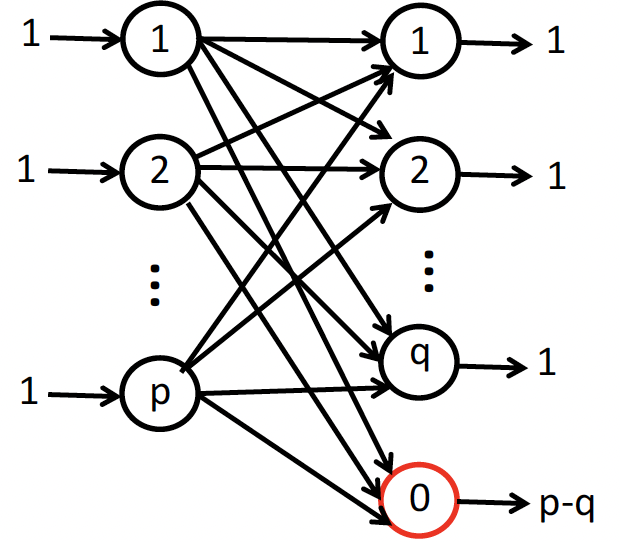
\includegraphics[width=0.56\columnwidth]{problem27.png}
\end{center}
\vspace{2pt}

\textbf{結果}: $m$個のsupply nodes（worker）と$n+1$個のdemand nodes（task + slack）\\
\textbf{正解}: D（$m$個のsupply nodes、$n+1$個のdemand nodes）

\textbf{Shortest Path Problem}: グラフ$G=(N,A)$で開始ノード$s$から終了ノード$t$への最短経路を求める。各アーク$(i,j)$の長さは$c_{ij} \geq 0$。

\textbf{定式化}:\\
$\min \sum c_{ij} x_{ij}$ s.t. フロー保存: $\sum_{(i,j)} x_{ij} - \sum_{(j,i)} x_{ji} = b_i$\\
$b_i = +1$ ($i=s$), $0$ ($i \neq s,t$), $-1$ ($i=t$), $x_{ij} \in \{0,1\}$

\textbf{ネットワークフロー問題として}:
\begin{itemize}
    \item 開始ノード$s$: supply = 1
    \item 終了ノード$t$: demand = 1
    \item その他のノード: supply/demand = 0（フロー保存）
    \item 完全単模性により、$x_{ij} \in \{0,1\}$の制約を外しても整数解が得られる
\end{itemize}

\mysection{PROBLEM 30: BRANCH-AND-BOUND TREE}

\vspace{2pt}
\begin{center}
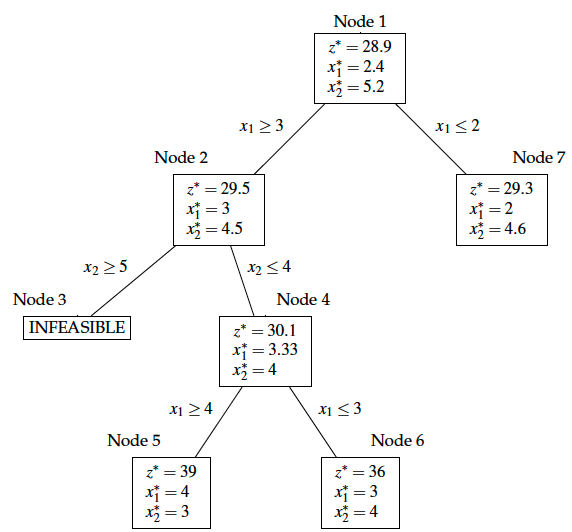
\includegraphics[width=0.85\columnwidth]{problem30.png}
\end{center}
\vspace{2pt}

\textbf{(a) 最小化か最大化か}: 最小化問題

\textbf{(b) 各ノードでさらに分枝が必要か}:
\begin{itemize}
    \item \textbf{Node 3}: 不要（実行不可能）
    \item \textbf{Node 5}: 不要（整数解あり）
    \item \textbf{Node 7}: 必要（分数解で、現在の上界より良い目的関数値）
\end{itemize}

\textbf{(c) 最適IP値の範囲}:
\begin{itemize}
    \item \textbf{下界}: 29.3（Node 7のLP緩和値）
    \item \textbf{上界}: 36（Node 6の整数解の値）
\end{itemize}
\textbf{理由}: 下界は未探索ノードのLP緩和値の最小値、上界は見つかった整数解の最良値

\mysection{重要ポイント・公式・性質まとめ}

\textbf{1. 線形計画法（LP）と双対性 (Duality)}
\begin{itemize}
    \item \textbf{弱双対性 (Weak Duality)}:
    \begin{itemize}
        \item 最小化問題（Primal）の任意の実行可能解の目的関数値は、最大化問題（Dual）の任意の実行可能解の目的関数値以上である（$c^T x \geq b^T y$）。
        \item \textbf{重要}: Primalが$-\infty$（非有界）なら、Dualは実行不可能。Dualが$+\infty$なら、Primalは実行不可能。
    \end{itemize}
    \item \textbf{強双対性 (Strong Duality)}:
    \begin{itemize}
        \item Primalが有限の最適解を持つなら、Dualも有限の最適解を持ち、両者の目的関数値は一致する（$c^T x^* = b^T y^*$）。
    \end{itemize}
    \item \textbf{相補性スラックネス (Complementary Slackness)}:
    \begin{itemize}
        \item 最適性の必要十分条件。$x$と$y$が最適であるためには以下が成立しなければならない：
        \item Primalの制約に余裕がある（$a_i^T x > b_i$）$\Rightarrow$対応するDual変数は0（$y_i = 0$）。
        \item Dual変数が正（$y_i > 0$）$\Rightarrow$対応するPrimal制約は等号で成立（Binding）している。
    \end{itemize}
    \item \textbf{可能性・不可能性のテーブル}:
    \begin{itemize}
        \item PrimalとDualが共に「有限最適値」を持つことは\textbf{あり得る}。
        \item PrimalとDualが共に「非有界（Unbounded）」になることは\textbf{あり得ない}（弱双対性に矛盾するため）。
        \item PrimalとDualが共に「実行不可能（Infeasible）」になることは\textbf{あり得る}。
    \end{itemize}
\end{itemize}

\textbf{4. 非線形・円錐計画 (Conic Programming)}
\begin{itemize}
    \item \textbf{特異値分解 (SVD)}:
    \begin{itemize}
        \item 任意の行列$A$は$A = U \Sigma V^T$と分解できる。
        \item \textbf{特異値$\sigma_i$の性質}: 常に非負である（$\sigma_i \geq 0$）。
        \item \textbf{固有値との関係}:
        \begin{itemize}
            \item 対称行列の場合：特異値は固有値の絶対値（$\sigma_i = |\lambda_i|$）。
            \item 一般行列の場合：$A^T A$の固有値は$\sigma_i^2$である。
        \end{itemize}
    \end{itemize}
    \item \textbf{低ランク近似 (Low Rank Approximation)}:
    \begin{itemize}
        \item 行列$A$に最も近いランク$r$の行列は、SVDで大きい順に$r$個の特異値を残すことで得られる（エッカート・ヤングの定理）。
    \end{itemize}
    \item \textbf{二次錐 (Second-Order Cone, SOC)}:
    \begin{itemize}
        \item アイスクリームコーンのような形。ノルム制約$\|x\|_2 \leq t$で定義される。
        \item \textbf{重要}: $t \geq 0$という条件が必須。これがないと凸集合にならない。
    \end{itemize}
\end{itemize}

\textbf{5. 離散最適化 (Discrete Optimization)}
\begin{itemize}
    \item \textbf{計算複雑性}:
    \begin{itemize}
        \item \textbf{クラスP}: 多項式時間で解ける問題（例：LP, SDP, SOCP）。
        \item \textbf{クラスNP}: 解が与えられたら、それが正しいか多項式時間で\textbf{検証}できる問題。
        \item \textbf{NP困難 (NP-Hard)}: 少なくともNPと同以上に難しい問題。離散最適化問題の多くはここに含まれる。
    \end{itemize}
    \item \textbf{モデリングのコツ}:
    \begin{itemize}
        \item \textbf{論理制約}: Binary変数$y \in \{0,1\}$と大きな数$M$ (Big-M)を使う。
        \begin{itemize}
            \item 「もし$x > 0$なら$y=1$」$\rightarrow$ $x \leq M y$。
            \item 「A または B」$\rightarrow$ $y_A + y_B \geq 1$。
        \end{itemize}
        \item \textbf{区分線形関数}: 凸でない関数も、Binary変数を使えばMIP（混合整数計画）として記述可能。
    \end{itemize}
\end{itemize}

\mysection{整数計画問題の要点まとめ}

\textbf{1. 「易しい」整数計画問題：ネットワークフロー}
\begin{itemize}
    \item \textbf{最小費用流問題}:
    \begin{itemize}
        \item 定義: ネットワーク上の各アークにコストと容量、各ノードで需給バランスを満たしつつ総コストを最小化
        \item \textbf{完全単模性}: 制約行列がネットワーク行列（各列に+1と-1が一つずつ）で、供給量$b_i$と容量$u_{ij}$が整数なら、全ての端点（基底実行可能解）は整数
        \item \textbf{結論}: 整数制約があってもLPで解けば自然に整数解が得られる
    \end{itemize}
    \item \textbf{応用例}: 最短路問題、割当問題も最小費用流の特殊ケース
\end{itemize}

\textbf{2. 「難しい」整数計画問題とモデリング技法}
\begin{itemize}
    \item \textbf{集合モデル}:
    \begin{itemize}
        \item \textbf{変数の定義（外科医の例）}:
        \begin{itemize}
            \item $m$: 手術タイプ（要素）の数
            \item $n$: 外科医（集合）の数
            \item $S_j$: 外科医$j$が実行できる手術タイプの集合
            \item $w_j$: 外科医$j$の重み（コストや能力など）
            \item $x_j \in \{0,1\}$: 外科医$j$を選ぶかどうか（1:選ぶ、0:選ばない）
        \end{itemize}
        
        \item \textbf{Set Packing}: 互いに素な集合を選び重み最大化\\
        $\max \sum w_j x_j$ s.t. $\sum_{j: i \in S_j} x_j \leq 1$ $\forall i$, $x_j \in \{0,1\}$\\
        各要素が高々1つの集合で選ばれる（0個でもOK、2個以上はNG）\\
        \textbf{例}: 外科医選択（各手術タイプを0人または1人の外科医でカバー、カバーされない手術タイプがあっても良い）
        
        \item \textbf{Set Covering}: 全要素をカバーする集合を選びコスト最小化\\
        $\min \sum w_j x_j$ s.t. $\sum_{j: i \in S_j} x_j \geq 1$ $\forall i$, $x_j \in \{0,1\}$\\
        各要素が少なくとも1つの集合でカバーされる\\
        \textbf{例}: 外科医選択（各手術タイプを少なくとも1人の外科医でカバー）← Problem 29
        
        \item \textbf{Set Partitioning}: 全要素を「ちょうど1回」カバー\\
        $\max/\min \sum w_j x_j$ s.t. $\sum_{j: i \in S_j} x_j = 1$ $\forall i$, $x_j \in \{0,1\}$\\
        各要素がちょうど1つの集合でカバーされる\\
        \textbf{例}: 外科医選択（各手術タイプをちょうど1人の外科医でカバー）
    \end{itemize}
    \item \textbf{施設配置問題}: 固定費と変動費、$x_j \leq M y_j$のリンク制約が重要
    \item \textbf{TSP}: 部分巡回路除去は指数関数的に存在。反復的に制約を追加するアプローチが有効
    \item \textbf{論理制約}: 最小稼働時間などもバイナリ変数で線形制約として記述可能
\end{itemize}

\textbf{3. 理論的枠組みと解法}
\begin{itemize}
    \item \textbf{LP緩和}:
    \begin{itemize}
        \item 整数制約を外して実数として解く
        \item 最小化問題で$v_{LP} \leq v_{IP}$（下界を与える）
        \item Optimality Gap: 上界と下界の差で最適性を評価
    \end{itemize}
    \item \textbf{分枝限定法}:
    \begin{itemize}
        \item LP緩和を解き、非整数変数で問題を分割（Branch）
        \item 枝刈り条件: 実行不可能、整数解発見、$v_{LP} \geq UB$
    \end{itemize}
\end{itemize}

\textbf{4. まとめ（アナロジー）}
\begin{itemize}
    \item \textbf{ネットワークフロー}: データが整数ならフローも自然と整数単位（LPで解ける「易しい」問題）
    \item \textbf{一般の整数計画}: LPで解くと「0.5個選ぶ」という非現実的答え。LP緩和で下界、分枝限定法で探索、強い定式化で範囲を狭める
\end{itemize}

\end{multicols}

\end{CJK}
\end{document}
